\documentclass[11pt,a4paper]{article}
\usepackage[T1]{fontenc}
\usepackage[utf8]{inputenc}
\usepackage{lmodern}
\usepackage[margin=2.5cm]{geometry}
\usepackage{amsmath,amssymb}
\usepackage{graphicx}
\usepackage{booktabs}
\usepackage{tabularx}
\usepackage{algorithm}
\usepackage{algpseudocode}
\usepackage[numbers,sort&compress]{natbib}
\usepackage[hidelinks]{hyperref}
\usepackage[capitalize]{cleveref}
\usepackage{caption}
\captionsetup{font=small,labelfont=bf}

%%%%%%%%% TITLE - PLEASE UPDATE TITLE HERE
\title{Adaptive Time Delay Stability (aTDS):\\letting the signals choose the window, lag range and tolerance}

\author{Asaf Markuza}
\date{}

\begin{document}

\maketitle

\begin{abstract}
Time Delay Stability (TDS) links two physiological signals when the delay that best aligns them stays nearly constant over consecutive windows. TDS has three parameters---the window, the lag range searched and the stability tolerance---counted in samples, with published values (60, $\pm30$, $\pm1$) chosen for sleep recordings at 1\,Hz. For any other time scale or sampling rate these values are a guess, and a fixed choice can fail silently: with a fixed $\pm30$ lag range, every coupled pair with a delay beyond 30 samples reported a wrong delay, in 16 of 50 cases with the wrong sign, at TDS scores of 72--96\,\%. Adaptive TDS (aTDS) sets all three parameters from the signals themselves: the window holds 30 independent samples of the slowest signal, the lag range is half the window (capped at half a rhythm period), and the tolerance is the widest value whose chance score on coupling-free, circularly rotated copies stays within a 5\,\% false-stability budget. On simulated signals with known coupling, aTDS restores detection where the published setting fails (AUC 0.92 vs 0.59 when the system is four times slower), reports the correct delay, and follows coupling that switches on and off and delays that drift. On real data, pyTDS reproduces the original TDS benchmark (43.53 vs 43.61\,\%); in 35 overnight polysomnograms aTDS detects the physiological network and reproduces the known sleep-stage pattern, agreeing with the published setting, which was designed for this data; on ECG and finger-pulse recordings of 53 intensive-care patients at 125\,Hz, data not analysed with TDS before to our knowledge, aTDS detects the heart-to-pulse coupling in 49 of 53 patients (AUC 0.95) where the published setting detects it in 14 (AUC 0.69); and in records from other fields it finds the known delays where the published setting does not---8\,h from rainfall to river flow and 1\,h from temperature to electricity demand. aTDS thus makes TDS usable, with a stated false-alarm budget, for any system and sampling rate.
%%%%%%%%% ABSTRACT %%%%%%%%%
\end{abstract}

\section{Introduction}
\label{sec:intro}
Physiological systems do not operate in isolation. The brain, heart, lungs, eyes and skeletal muscles continuously coordinate their activity, and the pattern of these interactions changes with physiological state. Network physiology studies this coordination by representing organ systems as nodes and their dynamical couplings as links of a time-varying network~\cite{Bashan2012NetworkPhysiology,Bartsch2015NetworkPhysiology,Ivanov2016FocusEmerging,Ivanov2021NewField}. The approach has shown that the network of organ interactions reorganises abruptly across sleep stages~\cite{Bashan2012NetworkPhysiology,Bartsch2015NetworkPhysiology}, that cardio-respiratory coupling undergoes transition-like changes between states~\cite{Bartsch2012PhaseTransitions}, that brain-wave interactions evolve across physiological states~\cite{Liu2015PlasticityBrain,Liu2015MajorComponent}, that the brain--muscle network is stratified by sleep stage~\cite{Rizzo2020NetworkPhysiology,Rizzo2022DynamicNetworks}, and that brain rhythms and heart rate interact with characteristic time delays~\cite{Lin2016DelaycorrelationLandscape}.

Most of these results rest on one pairwise coupling measure, Time Delay Stability (TDS)~\cite{Bashan2012NetworkPhysiology,Bartsch2015NetworkPhysiology}. TDS slides a window over two signals, finds in each window the time delay $\tau_0$ that maximises their cross-correlation, and declares the pair coupled for as long as $\tau_0$ stays nearly constant over consecutive windows. A window is labelled stable when at least 4 of 5 neighbouring delays agree within a tolerance, and the TDS score is the percentage of stable windows. The method is simple, interpretable and directly tied to a physical quantity, the delay, which is why it has become the standard tool of the field.

TDS, however, depends on three parameters counted in samples: the window length $L$, the lag range $\tau_{\max}$ searched, and the tolerance $\mathrm{tol}$. The published values, $L = 60$, $\tau_{\max} = \pm 30$ and $\mathrm{tol} = \pm 1$, were chosen for physiological series resampled to 1\,Hz. Because they are counted in samples, their meaning changes with both the time scale of the system and the sampling rate: the same physical coupling recorded at a sixteen-fold higher rate is seen by a 60-sample window through a sixteenth of the time span. For a new system there is no rule to choose them, and different implementations expose and set them differently, which makes TDS results hard to compare and reproduce~\cite{Steinbrinker2024TdspyOpensource}. A fixed choice can also fail silently. We show below that when the true delay lies outside a fixed $\pm30$ lag range, TDS still returns high scores (72--96\,\%) while reporting a wrong delay at the edge of the search, in 16 of 50 cases with the wrong sign: the TDS score measures how stable a delay is, not whether it is right.

We propose \emph{adaptive TDS} (aTDS), three rules that set the window, the lag range and the tolerance from the signals themselves, without knowing which pairs are coupled or what the delay is. The 4-of-5 stability rule of the original method is kept. The paper has four parts. Part~1 (\cref{sec:method}) explains the idea and the algorithm and shows, rule by rule, the tests that justify each choice. Part~2 (\cref{sec:simulation}) applies aTDS to simulated signals with known coupling and delay. Part~3 (\cref{sec:realdata}) applies it to real data: physiological recordings---the TDS benchmark pair and a 35-subject sleep cohort---and records from other fields with known delays (rivers, electricity demand, fuel prices). Part~4 (\cref{sec:conclusion}) summarises what aTDS is, why it is needed, and our verdict. All TDS computations use the open-source pyTDS implementation.

\subsection*{Related work}
\paragraph{Delay-based coupling measures in physiology.}
TDS was introduced to quantify how pairs of physiological signals lock onto a stable time delay and to build networks of organ interactions across sleep stages~\cite{Bashan2012NetworkPhysiology,Bartsch2015NetworkPhysiology}. Subsequent work used it to characterise brain-wave networks~\cite{Liu2015PlasticityBrain}, the dominant components of dynamic organ networks~\cite{Liu2015MajorComponent}, and cortico--muscular interactions~\cite{Rizzo2020NetworkPhysiology,Rizzo2022DynamicNetworks}, where TDS was computed in 60\,s windows moved in 30\,s steps~\cite{Rizzo2020NetworkPhysiology}. The delay-correlation landscape generalises the idea by examining the full profile of correlation against delay for brain--heart interactions~\cite{Lin2016DelaycorrelationLandscape}, and cardio-respiratory coupling has been shown to change abruptly between sleep stages~\cite{Bartsch2012PhaseTransitions}. In these studies the parameters are typically fixed in advance; the open-source TDSpy implementation exposes them as user parameters and notes that differing choices hamper reproducibility~\cite{Steinbrinker2024TdspyOpensource}. All of these methods inherit the classical theory of time-delay estimation by cross-correlation, whose accuracy depends on coherence and on the length of the observation window~\cite{Knapp1976GeneralizedCorrelation,Carter1987CoherenceTime}. Other coupling measures address different questions: Granger causality~\cite{Granger1969InvestigatingCausal} and transfer entropy~\cite{Schreiber2000MeasuringInformation} quantify directed predictive influence, convergent cross mapping~\cite{Sugihara2012DetectingCausality} targets coupling in nonlinear deterministic systems, and coupling-function methods reconstruct the form of interactions between oscillators~\cite{Stankovski2017CouplingFunctions}. These methods have their own embedding, lag and window parameters; aTDS is complementary to them and concerns the parameter choice of TDS itself.

\paragraph{Effective sample size of autocorrelated series.}
Bartlett showed that the variance of a correlation estimated between two autocorrelated series is inflated by a factor determined by the products of their autocorrelation functions~\cite{Bartlett1946TheoreticalSpecification}, and Bayley and Hammersley derived the corresponding effective number of independent observations of an autocorrelated series~\cite{Bayley1946EffectiveNumber}. These corrections are routinely used to adjust correlation tests in ecology~\cite{Pyper1998ComparisonMethods} and neuroimaging~\cite{Afyouni2019EffectiveDegrees}. In the TDS setting, the same reasoning implies that a fixed-length window carries fewer independent samples the slower the signals, so that the cross-correlation peak, and thus $\tau_0$, becomes unreliable. aTDS turns this observation into a design rule: it sets the window so that it always contains a fixed number of independent samples, using the Bartlett factor of each signal's autocorrelation.

\paragraph{Surrogate data and multiple testing.}
Surrogate data are the standard way to ask whether a statistic could have arisen without the property of interest~\cite{Theiler1992TestingNonlinearity,Schreiber2000SurrogateTime,Lancaster2018SurrogateData}. Phase-randomised and amplitude-adjusted surrogates preserve the spectrum and distribution of a series~\cite{Theiler1992TestingNonlinearity,Schreiber1996ImprovedSurrogate}; multivariate surrogates also preserve cross-spectra~\cite{Prichard1994GeneratingSurrogate}; and bivariate surrogates are needed to test for interdependence between two signals while keeping each signal's own structure~\cite{Andrzejak2003BivariateSurrogate}. The original TDS work builds its null by pairing signals across subjects within the same sleep stage~\cite{Bashan2012NetworkPhysiology}, which requires a cohort; we use it for our real sleep cohort (Section~5). aTDS uses a within-recording null, circular rotation of one signal relative to the other, which keeps both autocorrelations (exactly in the circular sense, and up to the wrap-around point otherwise) and applies to a single system; it uses this null twice, to calibrate the tolerance under a fixed false-stability budget and to obtain a per-link $p$-value. Because a network of $n$ signals involves $n(n-1)/2$ simultaneous tests, the per-link $p$-values are combined with the Benjamini--Hochberg procedure, which controls the expected proportion of false links among those reported~\cite{Benjamini1995ControllingFalse}.

\section{Part 1: the aTDS algorithm}
\label{sec:method}
\subsection{The idea}
\label{sec:idea}
\emph{The time scale matters---that is the point.} The right window, lag range and tolerance for TDS depend on how fast the signals change and how often they are sampled: a setting that fits 1-Hz sleep recordings is wrong for hourly river flow or for the same physiology sampled at 16\,Hz. In practice the user does not know this time scale in advance; they want to find out whether two signals are synchronised, and at what delay. aTDS removes the need to know it: the three parameters adjust themselves to whatever time scale and sampling rate the signals have.

TDS asks whether the delay between two signals stays stable. Whether it can answer depends on three numbers: how much data each window holds, how far it searches for the delay, and how much window-to-window wobble of the delay it accepts. aTDS sets each from the data, with one principle per number: the window must hold enough \emph{independent} samples of the slowest signal for its cross-correlation peak to be reliable; the lag range must be as wide as the window allows without aliasing; and the tolerance must be as wide as possible while coupling-free copies of the same signals stay below a fixed false-stability budget. No rule uses which pairs are coupled or the true delay.

\subsection{Time Delay Stability}
\label{sec:tds}
Given two signals $x$ and $y$, TDS splits them into windows $\nu = 1, \dots, N_w$ of length $L$ with step $s$ (50\,\% overlap in the original method). Within window $\nu$ both segments are z-scored and their circular (periodic-boundary) cross-correlation is computed,
\begin{equation}
C_\nu(\tau) = \frac{1}{L} \sum_{i=0}^{L-1} \tilde{x}_\nu\big((i+\tau) \bmod L\big)\, \tilde{y}_\nu(i), \qquad |\tau| \le \tau_{\max} ,
\label{eq:xcorr}
\end{equation}
and the delay is $\tau_0(\nu) = \arg\max_\tau |C_\nu(\tau)|$. A window is labelled \emph{stable} if it belongs to a run of 5 consecutive windows in which at least 4 delays lie within $\pm\mathrm{tol}$ of a common value. The TDS score is the percentage of stable windows~\cite{Bashan2012NetworkPhysiology,Bartsch2015NetworkPhysiology}. With the circular correlation of \cref{eq:xcorr}, lags beyond $(L-1)/2$ alias onto lags of the opposite sign, so $\tau_{\max} \le (L-1)/2$. In the implementation used here (pyTDS), a negative $\tau_0$ means that $x$ leads $y$.

\subsection{Overview of aTDS}
\begin{table}[t]
\centering
\caption{Notation and sign conventions.}
\label{tab:notation}
\footnotesize
\begin{tabularx}{\textwidth}{>{\raggedright\arraybackslash}p{2.6cm}>{\raggedright\arraybackslash}X}
\toprule
Symbol & Meaning \\
\midrule
$L$, $s$ & Window length and step (samples); $s = \lfloor L/2 \rfloor$. \\
$\tau_{\max}$ & Largest lag searched; $\tau_{\max} \le (L-1)/2$ under the circular correlation. \\
$\mathrm{tol}$ & Tolerance of the 4-of-5 stability rule (samples). \\
$\tau_0(\nu)$ & Lag of the largest $|C_\nu(\tau)|$ in window $\nu$; \textbf{negative $\tau_0$ means $x$ leads $y$}. \\
Reported delay & $-\tau_0$ (most frequent value among stable windows), so a \textbf{positive reported delay means $x$ leads}. \\
$B_i$, $B_{xy}$ & Bartlett factor of signal $i$ (\cref{eq:bartlett}) and joint factor $1 + 2\sum_k r_x(k)\,r_y(k)$ of a pair. \\
$C(t)$, $\mathrm{SE}(t)$ & Mean chance score of rotated copies at tolerance $t$ and its standard error. \\
$d_{\max}$ & Optional longest plausible delay supplied by the user. \\
$\tau_c$, $d$, $c$, $r$ & Correlation time, true delay, coupling strength and slow-down factor of the synthetic signals. \\
\bottomrule
\end{tabularx}
\end{table}
\Cref{tab:notation} collects the notation and sign conventions used throughout.

aTDS takes the $n$ signals $s_1, \dots, s_n$ of one system, each $T$ samples long, and returns one parameter set $(L, s, \tau_{\max}, \mathrm{tol})$ used for every pair, so that all scores of a network are measured on the same ruler. The stability rule (4 of 5 windows) is unchanged. The fixed design constants are: 30 independent samples per window, a 5\,\% false-stability budget, a window between 61 samples and 10\,\% of $T$, and 20 random rotations per pair (fewer when many pairs are pooled; \cref{sec:res-network}).

\subsection{Window}
\label{sec:window}
For each signal $i$ let $x_i = s_i - \bar s_i$ and
\begin{equation}
r_i(k) = \frac{\sum_t x_i(t)\, x_i(t+k)}{\sum_t x_i(t)^2}, \qquad k = 0, \dots, T/4 .
\end{equation}
With $K_i$ the first lag at which $r_i(k) \le 0$, the Bartlett factor is
\begin{equation}
B_i = 1 + 2 \sum_{k=1}^{K_i - 1} r_i(k)^2 .
\label{eq:bartlett}
\end{equation}
$B_i$ is the number of consecutive samples of signal $i$ that carry about as much information as one independent sample: $B = 1$ for white noise, and a window of $L$ samples holds $L / B_i$ independent samples. The window is
\begin{equation}
L = \operatorname{clip}\!\Big(\operatorname{round}\big(30 \cdot \max_i B_i\big),\; L_{\min},\; 0.1\,T\Big), \qquad s = \lfloor L/2 \rfloor ,
\label{eq:window}
\end{equation}
with $L_{\min} = 61$, or $\max(61, 2 d_{\max} + 1)$ if a longest plausible delay $d_{\max}$ is supplied; $L_{\min}$ takes precedence over the 10\,\% cap. The slowest signal sets the window, so every pair has at least 30 independent samples per window.

\emph{Why 30.} With $n$ independent samples each value of $C(\tau)$ has a random error of about $1/\sqrt{n}$, i.e.\ $\pm0.18$ at $n = 30$. Because $\tau_0$ is the maximum over roughly 30 independent lags, the largest pure-noise value is higher, about $0.18\sqrt{2\ln 30} \approx 0.47$, so a weak coupling does not stand out in every single window; it is the 4-of-5 rule that separates a peak returning to the same lag from noise peaks at random lags. More independent samples per window make $\tau_0$ more reliable but leave fewer windows and a coarser time resolution. The constant 30 is a convention that balances the two, not an optimum; \cref{sec:res-window} tests it.

\emph{Why 61.} The floor guarantees that the lag range is never narrower than the published $\pm30$.

\emph{What the window does not capture.} The Bartlett sum is truncated at the first zero crossing of the autocorrelation, so negative lobes are ignored, and for long-memory signals $B$ grows with the record length (\cref{sec:conclusion}); the window is therefore a property of the record as measured, not an intrinsic constant of the system. A user who needs a given time resolution can impose a maximum window; aTDS then sets the lag range and tolerance for that window.

\emph{Why the slowest signal, and not the pair.} For two independent series, Bartlett's formula gives the variance of their sample cross-correlation as approximately $\frac{1}{n}\big(1 + 2\sum_{k\ge1} r_x(k)\,r_y(k)\big)$~\cite{Bartlett1946TheoreticalSpecification}. By the Cauchy--Schwarz inequality,
\begin{equation}
\textstyle\sum_k r_x(k)\,r_y(k) \;\le\; \big(\sum_k r_x(k)^2\big)^{1/2}\big(\sum_k r_y(k)^2\big)^{1/2} \;\le\; \max_i \sum_k r_i(k)^2 ,
\end{equation}
so $\max_i B_i$ is an upper bound on this variance-inflation factor for every pair that can be formed from the signals; a window of $30\max_i B_i$ samples therefore holds at least about 30 independent samples for the cross-correlation of any pair, and one window puts all links of a network on the same ruler. Truncating the sums at the first zero crossing is a practical estimator choice, not part of Bartlett's result; it ignores later negative or seasonal lobes (\cref{sec:res-fields}). The joint factor $B_{xy} = 1 + 2\sum_k r_x(k)\,r_y(k)$ itself is the tighter, pair-specific alternative; in the one configuration we tested (\cref{tab:signals}) it gave the same detection with a window 2.8 times shorter, a tolerance 2.7 times tighter and a lower chance score (3.9\,\% vs 5.2\,\%).

\subsection{Lag range}
\label{sec:lag}
\begin{equation}
\tau_{\max} = \big\lfloor (L-1)/2 \big\rfloor, \qquad \tau_{\max} \leftarrow \max\!\big(1, \min(\tau_{\max}, \lfloor \min_i P_i / 2 \rfloor)\big),
\end{equation}
the cap applying only if some signal $i$ has a rhythm of period $P_i$.
The ratio $\tau_{\max} / L \approx 1/2$ is that of the published setting and the largest range the circular correlation of \cref{eq:xcorr} allows without aliasing. A signal is called rhythmic if, after the first zero crossing of $r_i$, the highest autocorrelation peak is at least 0.3 and not at the edge of the range; its lag is $P_i$. Beyond half a period, delays $d$ and $d - P$ cannot be told apart.

\subsection{Tolerance}
\label{sec:tol}
For each pair $(i, j)$ (at most 50 pairs, pooled over all recordings available, e.g.\ all subjects of a cohort), $s_j$ is circularly rotated by a random shift $h \in [a, T - a)$, $a = \max(L, \lfloor T/10 \rfloor)$, 20 times. Each rotated copy keeps both signals' autocorrelation but no coupling. For each copy $c$ the delay series is computed with the window and lag range above and scored with the 4-of-5 rule at tolerance $t$, giving $\mathrm{score}_c(t)$. The chance score and its standard error are
\begin{equation}
C(t) = \frac{1}{M}\sum_{c=1}^{M} \mathrm{score}_c(t), \qquad \mathrm{SE}(t) = \frac{\mathrm{SD}_c\big(\mathrm{score}_c(t)\big)}{\sqrt{M}} ,
\end{equation}
and the tolerance is
\begin{equation}
\mathrm{tol}^\ast = \max\big\{\, t \in \{0, 1, \dots, \max(1, \lfloor\tau_{\max}/4\rfloor)\} : C(t) + 2\,\mathrm{SE}(t) \le 5\,\% \big\}.
\label{eq:tol}
\end{equation}
Because a wider tolerance can only add stable windows, $C(t)$ is non-decreasing, so the scan stops at the first $t$ that exceeds the budget; the upper bound $C + 2\,\mathrm{SE}$ behaves the same way in practice. If even $t = 0$ exceeds it, the result is flagged \texttt{calibration\_failed}. The upper bound, rather than the mean alone, is used so that the budget also holds on new recordings; when the mean over 20 rotations of a single recording was used instead, the chance score on new pairs reached 6.7\,\%.

The 5\,\% is a design budget for false stability: on coupling-free data, at most 5\,\% of windows on average may be labelled stable. It is \emph{not} the probability that a link is false. The significance of an individual link still requires its own test (\cref{sec:res-network}).

\emph{Cost.} The calibration needs at most $50 \times 20 = 1\,000$ delay series of rotated copies. The delay series does not depend on the tolerance, so the scan over tolerances only re-applies the 4-of-5 rule to stored series; the dominant cost is therefore about 1\,000 sliding-window cross-correlation passes, independent of the number of tolerances tried.

\emph{How to read a score when the tolerance is wide.} The calibrated tolerance grows with the time scale, but in every setting of this paper it stays a small fraction of the lag range searched: from 4.5\,\% (rainfall--runoff, $\pm43$ of $\pm956$ samples) to 10.4\,\% ($r = 16$, $\pm56$ of $\pm541$), for example $\pm13$ of $\pm129$ in \cref{fig:example} and $\pm14$ of $\pm149$ in the capped sleep analysis. An aTDS score is therefore the share of windows in which the delay is stable to about one tenth of the range searched, and the delay itself is reported separately as the most frequent $\tau_0$ among stable windows. Because this resolution differs from the published $\pm1$ sample, aTDS scores are compared with the aTDS chance level of the same data, never with published TDS values.

\emph{Why widen the tolerance rather than lengthen the window.} Both reduce false instability: a longer window makes $\tau_0$ less jittery, a wider tolerance accepts the jitter. The oracle of \cref{sec:simulation} shows that, when time resolution does not matter, long windows with tolerance 0 detect best. aTDS instead fixes the window at 30 independent samples to keep time resolution and uses the tolerance, bounded by the chance budget, to absorb the remaining jitter.

\Cref{alg:atds} summarises the procedure.

\begin{algorithm}[t]
\caption{aTDS parameter selection}
\label{alg:atds}
\begin{algorithmic}[1]
\Require signals $s_1,\dots,s_n$ of length $T$; optional $d_{\max}$
\For{each signal $i$}
  \State $r_i \gets$ autocorrelation of $s_i$; \quad $K_i \gets$ first $k$ with $r_i(k)\le 0$
  \State $B_i \gets 1 + 2\sum_{k=1}^{K_i-1} r_i(k)^2$
\EndFor
\State $L_{\min} \gets 61$ (or $\max(61, 2d_{\max}+1)$ if $d_{\max}$ given)
\State $L \gets \operatorname{clip}(\operatorname{round}(30\max_i B_i), L_{\min}, 0.1T)$ \Comment{$L_{\min}$ wins if $0.1T<L_{\min}$}
\State $s \gets \lfloor L/2\rfloor$; \quad $\tau_{\max} \gets \lfloor (L-1)/2 \rfloor$
\If{some signals are rhythmic with periods $P$} $\tau_{\max} \gets \max(1, \min(\tau_{\max}, \lfloor\min P/2\rfloor))$ \EndIf
\State $\mathcal{N} \gets$ delay series of $(s_i, \mathrm{rotate}(s_j, h))$ for $\le 50$ pairs $\times$ 20 shifts $h$, all recordings
\State $\mathrm{tol} \gets 0$
\For{$t = 0, 1, \dots, \max(1, \lfloor \tau_{\max}/4\rfloor)$}
  \State $C, \mathrm{SE} \gets$ mean and standard error of 4-of-5 TDS scores of $\mathcal{N}$ at tolerance $t$
  \If{$C + 2\,\mathrm{SE} \le 5\,\%$} $\mathrm{tol} \gets t$ \Else\ \textbf{break} \EndIf
\EndFor
\State \Return $L$, $s$, $\tau_{\max}$, $\mathrm{tol}$; flag \texttt{calibration\_failed} if $C + 2\,\mathrm{SE} > 5\,\%$ at $t=0$
\end{algorithmic}
\end{algorithm}

The rules never use which pairs are coupled or the true delay. They are not entirely blind to coupling, however: a coupled signal's autocorrelation partly reflects its partner.


\subsection{How each rule was tested}
\label{sec:tests}
Each rule was tested on simulated signals whose coupling and delay are known, changing only that rule and keeping the others fixed. The signals and metrics are described here; Part~2 uses the same design.

\label{sec:design}
\paragraph{Signals.} The main test signal is an AR(1) process $x$ with correlation time $\tau_c$ ($\phi = e^{-1/\tau_c}$), z-scored, with partner $y(t) = c\, x(t-d) + \sqrt{1-c^2}\,\eta(t)$, where $\eta$ is an independent AR(1) process with the same $\tau_c$; uncoupled pairs use $c = 0$. Further signal classes are fractional Gaussian noise with Hurst exponent $H$ generated by circulant embedding (long memory, $H$ equal to the DFA exponent~\cite{Peng1995QuantificationScaling}), AR(2) oscillators with period 40 and pole radius 0.97 (rhythms), two Rulkov map neurons~\cite{Rulkov2002ModelingSpikingbursting} with delayed diffusive one-way coupling (bursts), mixed-speed systems, and a record whose memory changes from $\tau_c = 4$ to 16 halfway. Records are 20\,000 samples unless stated otherwise (30\,000 for the pair of \cref{fig:example,fig:tol} and for \cref{fig:window}a; 40\,000 for the on/off test; 6\,000 for Rulkov; 10\,000 for networks). The real recording is the sleep-EEG $\delta$- and $\sigma$-band power pair at 1\,Hz distributed with pyTDS.

\paragraph{Slow-down factor.} To emulate the same system recorded at a higher rate, a system is slowed by a factor $r$: memory $\tau_c = 2r$ and delay $d = 5r$ samples. At $r = 1$ the published setting fits; the larger $r$, the worse it fits.

\paragraph{Settings compared.} \emph{Published}: $L = 60$, $s = 30$, $\tau_{\max} = \pm30$ ($\pm29$ effective under \cref{eq:xcorr}), $\mathrm{tol} = \pm1$. \emph{Rescaled by hand}: the published setting multiplied by the true $r$ ($60r$, $30r$, $\pm30r$, $\pm r$); fair but generous, since $r$ is unknown in real data. \emph{aTDS}: as in \cref{sec:method}, not told $r$. \emph{Oracle}: the best of up to 91 settings (7 windows from 30 to 1\,920 samples with $\tau_{\max} = (L-1)/2$, $\times$ 13 tolerances from 0 to 135), chosen by AUC on 20 coupled and 20 uncoupled labelled training pairs; a practical upper bound that no real analysis can use.

\paragraph{Train/test separation.} aTDS sets its parameters on separate training data that are not scored: 5 training pairs in the synthetic tests and the first half of the record for the EEG pair. In the network test calibration is label-free on the scored network itself, as in a real analysis.

\paragraph{Metrics.} \emph{AUC}: the probability that a coupled pair outscores an uncoupled one~\cite{Hanley1982MeaningUse}, with 95\,\% intervals from 1\,000 bootstrap resamples of the pairs~\cite{Efron1979BootstrapMethods}, paired across methods for differences. \emph{Delay found}: the share of coupled pairs with at least 3 stable windows whose median $\tau_0$ lies within 10\,\% (at least $\pm1$ sample) of the true delay, with Wilson intervals~\cite{Wilson1927ProbableInference}. \emph{Better / equivalent / undecided}: for two methods on the same pairs, ``better'' if the 95\,\% interval of the AUC difference lies above 0; ``equivalent'' if its 90\,\% interval lies inside $\pm0.05$ (two one-sided tests~\cite{Schuirmann1987ComparisonTwo}); otherwise ``undecided''. \emph{Chance score}: the mean TDS score of uncoupled pairs or rotated copies.

\paragraph{Implementation.} TDS is computed with pyTDS (circular cross-correlation, z-scored windows, $\tau_0 = \arg\max|C|$, 4-of-5 rule, default non-causal stability anchor). All seeds are fixed. The scripts behind every figure and table, and their raw outputs, are in the repository (see Code and data availability).


\subsection{A motivating example}
\label{sec:example}
\Cref{fig:example} shows one coupled pair ($\tau_c = 8$, $d = 20$, $c = 0.6$) analysed with the published setting and with the parameters aTDS chose on a separate training pair of the same kind ($L = 259$, $\tau_{\max} = \pm129$, $\mathrm{tol} = \pm13$). With the fixed window $\tau_0$ scatters and rarely holds for 4 of 5 windows: the TDS score is 5.2\,\%, with $\tau_0$ within $\pm2$ samples of the true delay in 28\,\% of windows. With aTDS, $\tau_0$ sits on the true delay: the score is 91.3\,\%, with $\tau_0$ within $\pm2$ samples in 90\,\% of windows. The coupling is identical; only the parameters differ.

\begin{figure}[t]
\centering
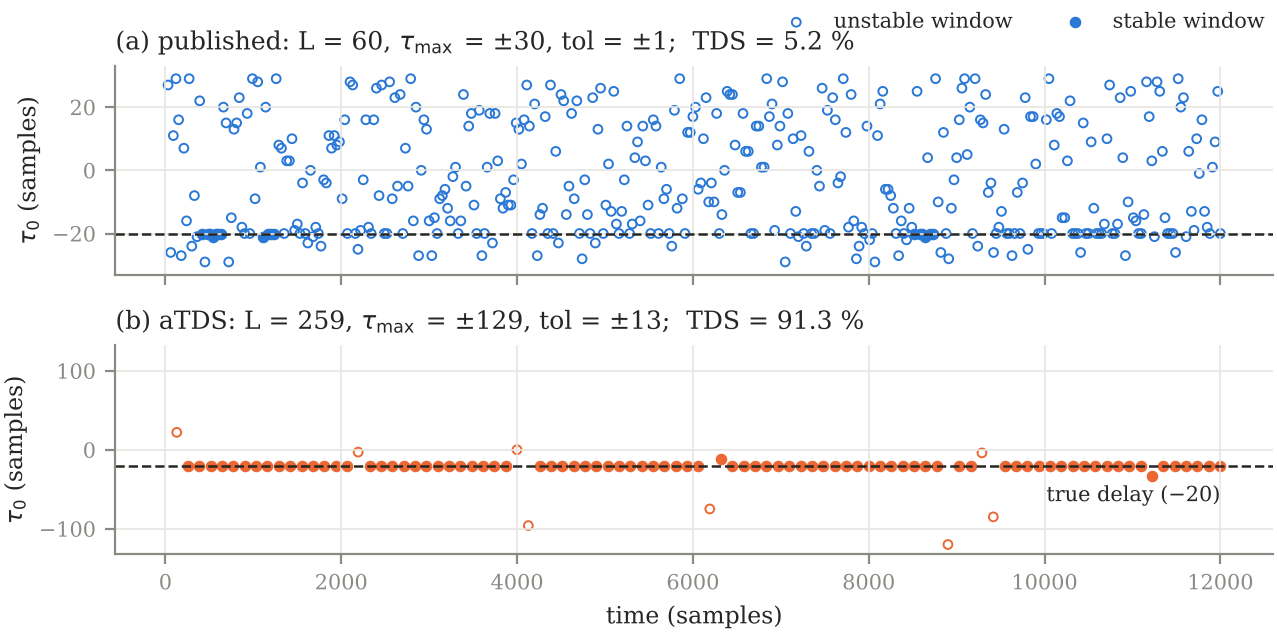
\includegraphics[width=\textwidth]{figures/fig_example_fixed_vs_atds.png}
\caption{The same coupled pair ($\tau_c = 8$, true delay 20 samples, coupling 0.6) under the published fixed parameters (a) and the parameters chosen by aTDS on a separate training pair (b). Each dot is $\tau_0$ in one window over the first 12\,000 samples; filled dots are stable windows. The dashed line is the true delay ($\tau = -20$; negative means $x$ leads).}
\label{fig:example}
\end{figure}


\subsection{Test of the window rule}
\label{sec:res-window}
A fixed 60-sample window holds fewer independent samples the slower the signal, down to 0.93 at $\tau_c = 64$ (\cref{fig:window}a); the aTDS window holds 30 by construction. \Cref{fig:window}b varies only the window for two weakly coupled systems ($c = 0.3$): a faster one ($\tau_c = 4$, $d = 10$) and one four times slower ($\tau_c = 16$, $d = 40$), with $\tau_{\max} = (L-1)/2$ and the tolerance calibrated at every window length. aTDS chose 121 and 515 samples respectively, about four times longer for the four-times slower system, reaching AUC 0.97 [0.95, 0.99] and 0.79 [0.73, 0.85] against 0.83 and 0.51 at 60 samples. Detection keeps rising past the aTDS choice (0.99 at 1\,920 samples for the slower system): with coupling that is always on, a longer window is always better, so the aTDS window is a compromise with time resolution rather than the best window for detection.

\begin{figure}[t]
\centering
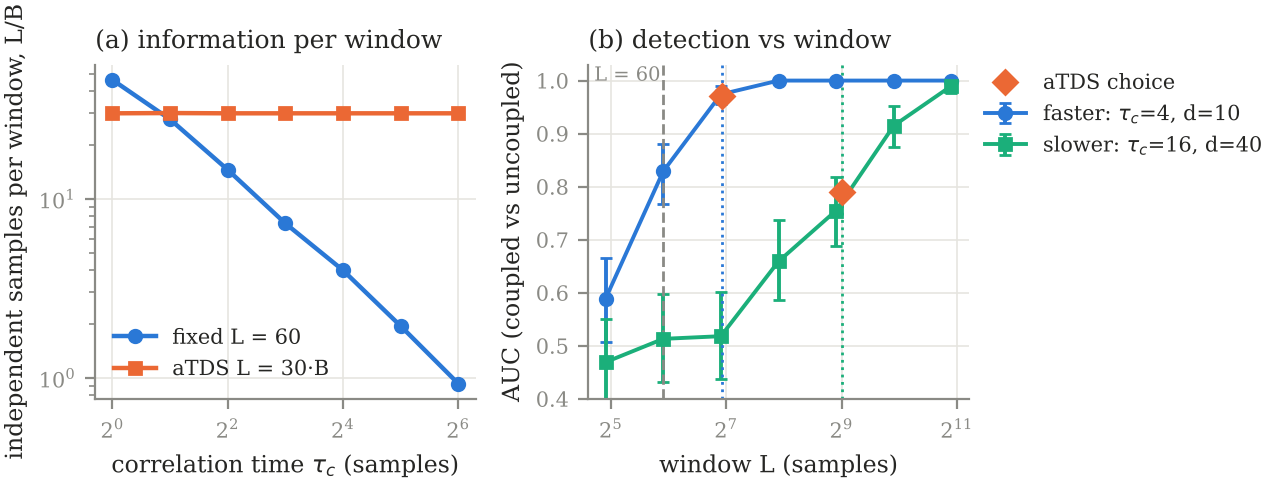
\includegraphics[width=\textwidth]{figures/fig_window_rule.png}
\caption{Window rule. (a) Independent samples per window, $L/B$, against the correlation time $\tau_c$ (median $B$ over 5 signals of 30\,000 samples). (b) AUC against window length for a faster and a four-times slower system with weak coupling (100 coupled and 100 uncoupled pairs per point; bootstrap 95\,\% intervals). Dotted lines and diamonds: the window chosen by aTDS for each system; dashed line: $L = 60$.}
\label{fig:window}
\end{figure}

To test the constant 30 when time resolution matters, coupling ($c = 0.6$, $\tau_c = 8$, $d = 20$) was switched on and off in blocks of 1\,000, 2\,000 or 4\,000 samples (40\,000 samples, 20 pairs per point). A window counts as correct if, during coupling, it is stable with $\tau_0$ within $\pm2$ samples of the true delay, or, without coupling, it is not stable. \Cref{fig:onoff} shows a real trade-off whose optimum depends on episode length: 45 independent samples for the shortest blocks (balanced accuracy 0.87; 30 gives 0.85), 60 for 2\,000-sample blocks (0.92; 30 gives 0.88), and a plateau of 0.94--0.95 from 45 on for the longest blocks (30 gives 0.91). The aTDS constant is within 0.015--0.05 of the best in all three cases, on the short side.

\begin{figure}[t]
\centering
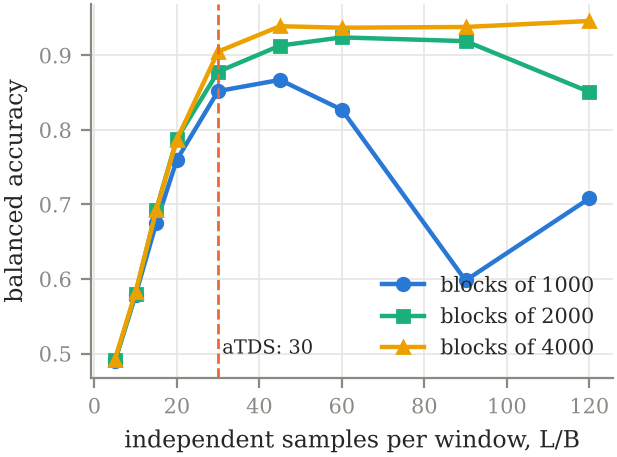
\includegraphics[width=0.55\textwidth]{figures/fig_onoff_tradeoff.png}
\caption{Coupling switched on and off in blocks of 1\,000--4\,000 samples. Balanced accuracy of the window labels against the number of independent samples per window; dashed line: the aTDS constant 30.}
\label{fig:onoff}
\end{figure}


\subsection{Test of the lag-range rule}
\Cref{fig:lag} isolates the lag range. Slow coupled signals ($\tau_c = 16$, $c = 0.6$) with true delays from 5 to 160 samples (10 pairs per delay) were scored with the aTDS window and tolerance (windows 454--514, tolerances $\pm23$ to $\pm29$) and either the published $\pm30$ or the aTDS range $(L-1)/2$ ($\pm226$ to $\pm256$). With the aTDS range the reported delay is exact for all 90 pairs, sign included. With $\pm30$, all 50 pairs with delays beyond 30 report a wrong delay at the edge of the search ($\pm30$, once 18), 16 of them with the wrong sign, while their TDS scores stay high (72--96\,\%). A high TDS score can therefore coexist with a wrong delay when the lag range is fixed. aTDS scores fall at long delays (27--62\,\% at $d = 160$) because the overlap of $x$ and delayed $y$ within a window shrinks; the delay reported from the stable windows remains right. Within $\pm30$ both variants are right and the narrow range scores somewhat higher (94--100\,\% vs 82--99\,\%), as it has fewer lags to pick wrongly by chance.

\begin{figure}[t]
\centering
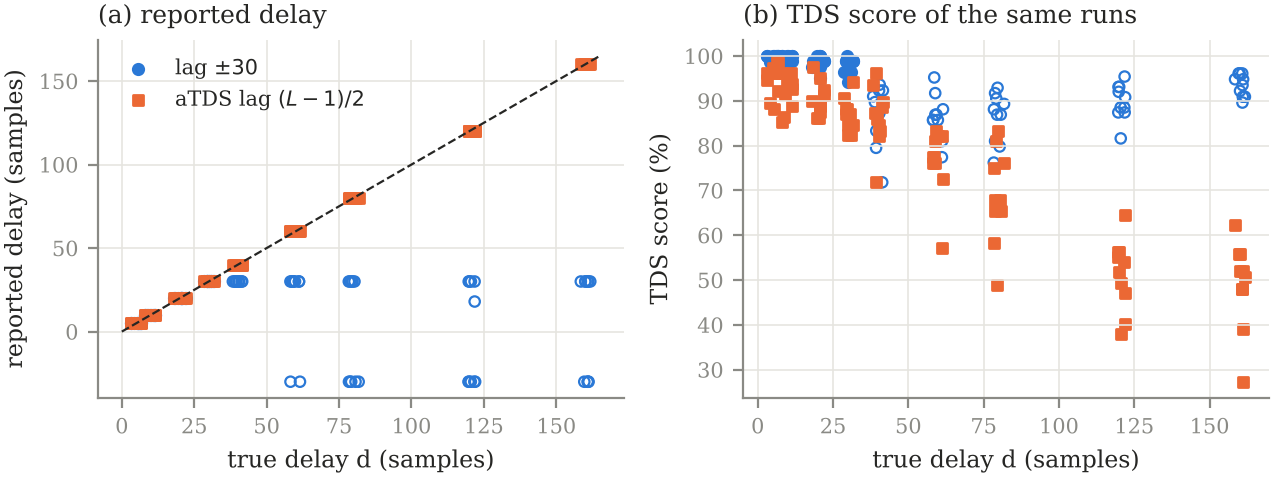
\includegraphics[width=\textwidth]{figures/fig_lag_range.png}
\caption{Only the lag range changes. (a) Reported delay ($-\tau_0$, with $\tau_0$ the most frequent value among stable windows; positive means $x$ leads) against the true delay; the dashed diagonal is a perfect answer. (b) TDS score of the same runs. Filled markers: right delay; hollow: wrong delay. Points are jittered horizontally.}
\label{fig:lag}
\end{figure}


\subsection{Test of the tolerance rule}
\Cref{fig:tol}a shows the calibration on the example pair: the chance score of 20 rotated copies rises with the tolerance, and its upper bound crosses 5\,\% between $\pm12$ and $\pm13$; aTDS chose $\pm13$ from rotations of its training pairs. On the real pair (\cref{fig:tol}b) the score barely depends on the tolerance (90.0\,\% at 0, 91.3\,\% at $\pm13$), so the gain in \cref{fig:example} comes from the window and lag range. The tolerance caps false stability while allowing the delay to wobble.

\begin{figure}[t]
\centering
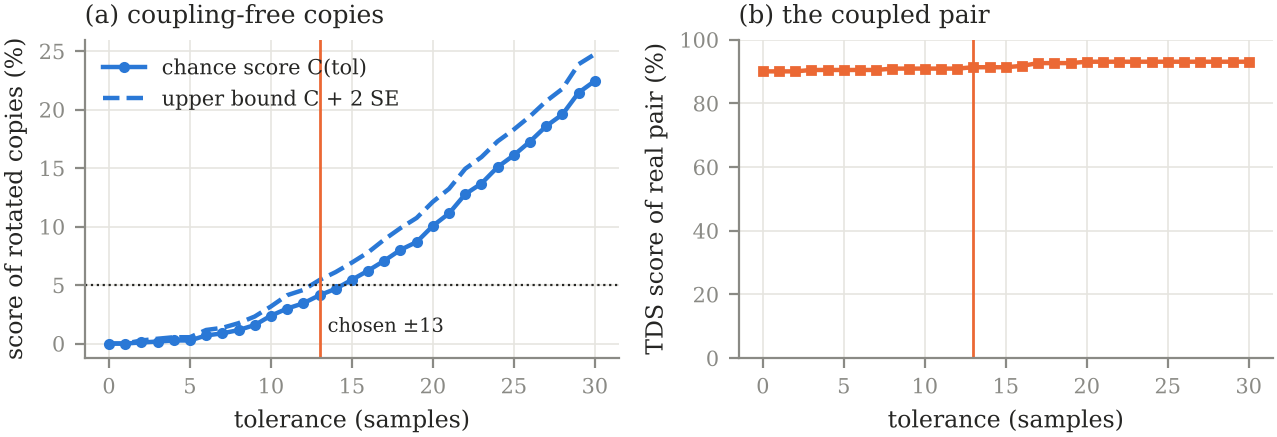
\includegraphics[width=\textwidth]{figures/fig_tolerance_calibration.png}
\caption{Tolerance calibration for the pair of \cref{fig:example} with the aTDS window. (a) Chance score $C(\mathrm{tol})$ of circularly rotated copies and its upper bound $C + 2\,\mathrm{SE}$; dotted line: 5\,\% budget. (b) TDS score of the real, unrotated pair at the same tolerances.}
\label{fig:tol}
\end{figure}

With the aTDS window and lag range fixed and only the tolerance changed ($\pm1$ vs calibrated; slow-down test, $c = 0.3$, 100 + 100 pairs per $r$), calibration helps slow systems recover the delay: 85\,\% vs 66\,\% of coupled pairs at $r = 8$ (intervals do not overlap), 88\,\% vs 77\,\% at $r = 4$ and 42\,\% vs 26\,\% at $r = 16$ (intervals overlap). The AUC gain ($+0.04$ at $r = 4$ and 8) is not significant at 95\,\%, and at $r = 1$ the calibrated tolerance is very slightly worse ($-0.005$, interval $-0.012$ to $-0.001$). The gain comes from having enough stable windows: with $\pm1$ only 77, 66 and 26 of 100 coupled pairs at $r = 4, 8, 16$ have 3 or more stable windows (almost all of them right), whereas with calibration 98, 93 and 53 have them, of which 90, 91 and 79\,\% are right. The mean chance score on new pairs is 3.3--4.4\,\% at every $r$, inside the budget.


\section{Part 2: simulated data}
\label{sec:simulation}
\subsection{All three rules together: the slow-down test}
\Cref{fig:slowdown} and \cref{tab:slowdown} compare the four settings across the slow-down test. aTDS is far better than the published setting once the system is slower than that setting assumes (AUC 0.92 vs 0.59 at $r = 4$; 95\,\% interval of the difference $+0.24$ to $+0.42$); the published setting is close to chance from $r = 4$ on. Against the setting rescaled by hand, with a $\pm0.05$ equivalence margin, aTDS is equivalent at $r = 1$ and 2 (the rescaled setting is marginally higher at $r = 2$, 0.99 vs 0.98), better at $r = 8$ (0.88 vs 0.81; interval of the difference $+0.007$ to $+0.142$; delay found in 85\,\% vs 60\,\% of pairs) and undecided at $r = 4$ and 16 (90\,\% intervals $-0.064$ to $+0.003$ and $-0.105$ to $+0.018$). The oracle is better than aTDS at every $r \ge 2$, mostly by choosing much longer windows. The upper-bound tolerance rule costs some detection at $r = 16$ (AUC 0.65, against 0.72 when the tolerance was set from the mean chance score of a single recording, and 0.69 for the rescaled setting).

\begin{figure}[t]
\centering
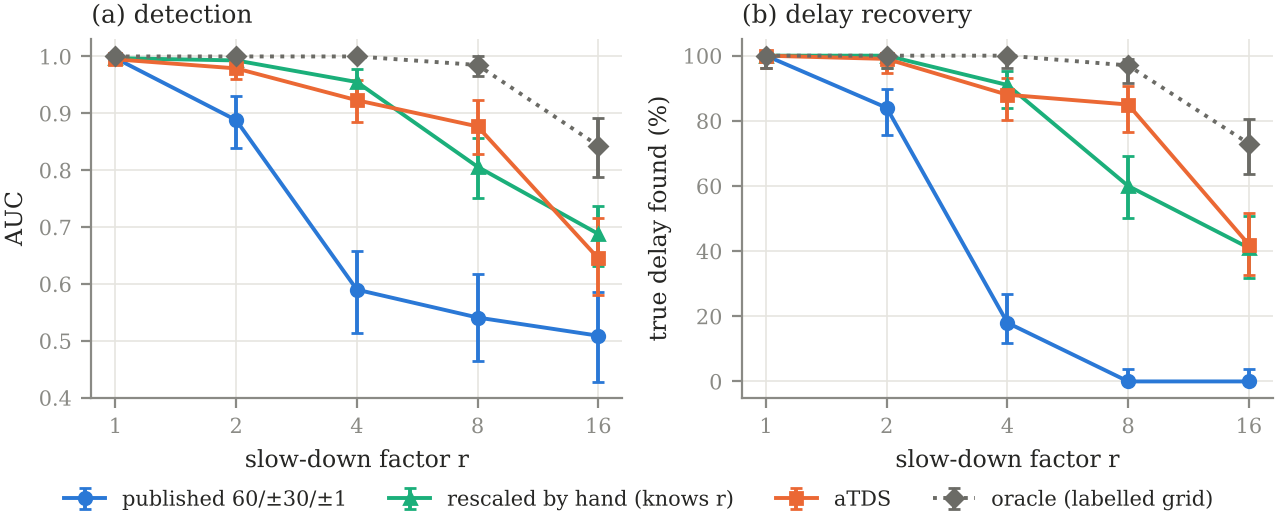
\includegraphics[width=\textwidth]{figures/fig_slowdown_baselines.png}
\caption{Slow-down test ($\tau_c = 2r$, $d = 5r$, coupling 0.3; 100 coupled and 100 uncoupled pairs per $r$). (a) AUC with bootstrap 95\,\% intervals. (b) Share of coupled pairs whose stable windows report the true delay, with Wilson 95\,\% intervals. The rescaled setting is given the true $r$; the oracle tunes on labelled pairs; aTDS is given neither.}
\label{fig:slowdown}
\end{figure}

\begin{table}[t]
\centering
\caption{Slow-down test: AUC [95\,\% interval] and parameters chosen. Window / lag / tolerance in samples.}
\label{tab:slowdown}
\resizebox{\textwidth}{!}{%
\begin{tabular}{rcccccc}
\toprule
$r$ & Published & Rescaled & aTDS & Oracle & aTDS parameters & Oracle parameters \\
\midrule
1  & 0.997 [0.989, 1.00] & 0.997 [0.989, 1.00] & 0.995 [0.988, 1.00] & 1.000 [0.999, 1.00] & 66 / 32 / 3     & 60 / 29 / 0 \\
2  & 0.888 [0.839, 0.93] & 0.993 [0.984, 1.00] & 0.979 [0.961, 0.99] & 1.000 [1.00, 1.00] & 126 / 62 / 6    & 240 / 119 / 0 \\
4  & 0.590 [0.513, 0.66] & 0.955 [0.926, 0.98] & 0.923 [0.885, 0.96] & 1.000 [1.00, 1.00] & 237 / 118 / 12  & 960 / 479 / 0 \\
8  & 0.541 [0.464, 0.62] & 0.806 [0.752, 0.86] & 0.877 [0.829, 0.92] & 0.985 [0.965, 1.00] & 563 / 281 / 27  & 1920 / 959 / 0 \\
16 & 0.509 [0.428, 0.59] & 0.688 [0.631, 0.74] & 0.645 [0.580, 0.72] & 0.843 [0.788, 0.89] & 1083 / 541 / 56 & 1920 / 959 / 135 \\
\bottomrule
\end{tabular}}
\end{table}


\subsection{Other signal classes}
\Cref{tab:signals} runs aTDS against the published setting on signal classes typical of physiology. In every row aTDS set its parameters on data that were not scored. aTDS is better for strongly long-memory signals ($H = 0.9$), rhythms with delays below half a period, changing dynamics and Rulkov neurons, and equal or not distinguishable for $H = 0.6$ and 0.75. For a rhythm with a delay beyond half a period the coupling is detected but the delay is wrong, as expected from the lag cap. For a fast signal with a long delay (50 samples), the default lag range ($\pm30$) is too short and the optional $d_{\max}$ is needed.



Two rows point to refinements. In a mixed-speed network, a single window set by the slowest signal gives fast pairs a wide tolerance ($\pm56$ instead of $\pm3$ with a per-pair window). For a coupled fast--slow pair, the joint Bartlett factor $B_{xy} = 1 + 2\sum_k r_x(k)\, r_y(k)$ (11.3, between $B_x = 31.3$ and $B_y = 5.0$) gave the same detection with a window 2.8 times shorter and a tolerance 2.7 times tighter than the max-$B$ rule. For Rulkov neurons the delay was reported a constant 3 steps too long at both delays, probably the map's response latency; calibration did not fail under one-way coupling.


\begin{table}[t]
\centering
\caption{Other signal classes with known answers. AUC with bootstrap 95\,\% intervals where available; ``found'': share of coupled pairs with the true delay.}
\label{tab:signals}
\footnotesize
\begin{tabularx}{\textwidth}{>{\raggedright\arraybackslash}p{3.4cm}>{\raggedright\arraybackslash}X>{\raggedright\arraybackslash}X>{\raggedright\arraybackslash}X}
\toprule
Signals & Published 60 / $\pm30$ / $\pm1$ & aTDS & Reading \\
\midrule
fGn $H = 0.6$, $d = 20$, $c = 0.2$ & AUC 0.60 [0.47, 0.72], found 28\,\% & 0.59 [0.45, 0.71], 23\,\% ($L = 61$) & Equal \\
fGn $H = 0.75$, $d = 20$, $c = 0.2$ & 0.70 [0.59, 0.81], 33\,\% & 0.65 [0.53, 0.77], 23\,\% ($L = 73$) & Not distinguishable \\
fGn $H = 0.9$, $d = 20$, $c = 0.2$ & 0.46 [0.33, 0.58], 15\,\% & 0.82 [0.73, 0.91], 85\,\% ($L = 614$, $\pm34$) & aTDS better; $B$ grows with record length \\
Rhythm $P \approx 40$, $d = 8$ & 0.97, 43\,\% & 1.00, 100\,\% (period 41, lag $\pm20$) & aTDS better \\
Rhythm $P \approx 40$, $d = 30$ & 0.46, 0\,\% & 0.995, 0\,\% (reports 11) & Detected, delay wrong (anti-phase lobe) \\
Rulkov neurons, $d = 16$ / 32 & 0.73 / 0.79; median delay 0 / 15.5 & 1.00 / 1.00; median delay 19 / 35 & aTDS better; constant $+3$ offset \\
Fast ($\tau_c = 1$), $d = 50$, $c = 0.5$ & 0.56, 0\,\% & default ($L = 61$): 0.56, 0\,\%; with $d_{\max} = 60$ ($L = 121$): 1.00, 100\,\% & Needs optional $d_{\max}$ \\
Memory $\tau_c$ 4 $\to$ 16, $d = 10$, $c = 0.4$ & 1st half 0.98; 2nd half 0.71, 45\,\% & one window (252): 1.00 / 0.96, 90\,\%; per half (124 / 484): 1.00 / 0.98, 100\,\% & aTDS better; per segment slightly better \\
Mixed: slow ($\tau_c$ 32, $d = 40$) + fast ($\tau_c$ 2, $d = 5$) pair & slow 0.44, fast 1.00 & one window (972): 0.99 / 1.00, fast tol $\pm56$; per-pair: fast $L = 64$, $\pm3$ & System-wide window costs fast-pair precision \\
Slow $x$ ($\tau_c$ 32) drives fast $y$ ($\tau_c$ 2), $d = 10$ & 0.83, 57\,\% & max-$B$ window (939, $\pm51$): 1.00, 100\,\%; joint $B_{xy}$ (339, $\pm19$): 1.00, 100\,\% & Joint $B_{xy}$: same detection, 2.8$\times$ shorter window \\
\bottomrule
\end{tabularx}
\end{table}

\subsection{Networks: per-link significance with FDR control}
\label{sec:res-network}
The 5\,\% budget bounds the mean chance score, not the false-positive rate of an individual link. For networks we therefore combine aTDS with a per-link rotation test: a link's $p$-value is $(1 + \#\{\text{rotations scoring} \ge \text{the real score}\}) / 1\,000$ over 999 rotations, and the 15 links of a six-signal network are tested together with the Benjamini--Hochberg procedure at $q = 0.05$~\cite{Benjamini1995ControllingFalse}. Two designs ($\tau_c = 8$, 10\,000 samples, coupling 0.4; 10 coupled and 10 uncoupled networks each) were tested: three disjoint links ($0\to1$, $2\to3$, $4\to5$; delays 10, 20, 15) and a common driver (0 drives 1 with delay 10 and 2 with delay 20, plus $3\to4$ with delay 15), which induces an indirect 1--2 link. aTDS set one parameter set per network by rotation only, without labels (tolerance calibrated on 4 rotations of each of the 15 pairs, 60 in total).

The per-link test was calibrated: on uncoupled links 2.7--5.8\,\% reached $p \le 0.05$. After FDR control no false link appeared in any of the 20 uncoupled networks. In the coupled networks aTDS found 27 of 30 true links (disjoint) and 26 of 30 (common driver), with a mean false-discovery proportion of 8.3\,\% and 2.5\,\%. With only 10 networks per design these proportions are imprecise, and the 8.3\,\% of the disjoint design, above the 5\,\% target, should be read as inconclusive rather than as a failure or a confirmation of FDR control. The indirect link of the common driver was not reported in any network (raw $p \le 0.05$ in 1 of 10); at coupling 0.4 the indirect correlation is only about $0.4 \times 0.4 = 0.16$. Pairwise TDS cannot distinguish indirect from direct links, so with stronger drivers indirect links are expected to appear.


\subsection{Coupling that switches, drifts or is nonlinear}
\label{sec:res-hard}
\paragraph{Coupling that switches with the regime.} The sleep-stage situation, in which both the coupling and the signals' own dynamics change from one regime to the next, was simulated with blocks of 2\,000 samples alternating between regime A ($\tau_c = 8$, $y$ follows $x$ with delay 20 and coupling 0.6) and regime B ($\tau_c = 32$, uncoupled), with uncoupled controls (40 + 40 pairs, 20\,000 samples, regimes scored with the 80\,\% purity rule of \cref{sec:res-cohort}). The published setting labelled only 5.6\,\% of regime-A windows stable (controls 0.7\,\%; AUC 0.944, delay found in 95\,\% of pairs), aTDS 98.9\,\% (controls 4.4\,\%; AUC 1.0, delay found in all pairs; window 516, tolerance $\pm29$), and aTDS with parameters set per regime 84.3\,\% (AUC 1.0). The price is false stability in the uncoupled regime: 8.1\,\% for aTDS and 9.0\,\% per regime (controls 5.8\,\% and 4.5\,\%), above the 5\,\% budget, against 0.9\,\% for the published setting. Windows near a regime boundary inherit the stable delay of the coupled regime; with long windows, regime-resolved scores need a boundary margin. Excluding windows that lie within one window length of a regime boundary removes most of this leak: aTDS's false stability in the uncoupled regime fell from 8.1 to 3.8\,\% for coupled pairs, within the budget, although the controls stayed slightly above it (5.5\,\%), at unchanged AUC. For regime-limited coupling, windows must be short relative to the regimes.

\paragraph{Nonlinear coupling.} With monotone coupling, $y = 0.6\,\tanh(2x(t-d))/\mathrm{sd} + $ noise ($\tau_c = 8$, $d = 20$, 100 + 100 pairs), both settings are near perfect (published AUC 0.997, aTDS 1.0). With non-monotone coupling, $y \propto x(t-d)^2 - 1$, for which the linear correlation is zero by construction, the published setting reached AUC 0.803 (delay found 74\,\%) and aTDS 0.747 (62\,\%): TDS detects such coupling only through local, window-wise correlation, and aTDS's longer windows average it out. Correlation-based TDS is not designed for non-monotone coupling, and aTDS does not help there.

\paragraph{Drifting delay.} With a delay drifting linearly from 10 to 30 samples ($\tau_c = 8$, coupling 0.6, 40 pairs), the published setting labelled 8.5\,\% of windows stable and aTDS 86.5\,\%; both tracked the delay closely in their stable windows (median absolute error 0.30 and 0.25 samples). aTDS follows a slowly drifting delay through nearly the whole record.
%%%%%%%%% SIMULATION %%%%%%%%%

\section{Part 3: real data}
\label{sec:realdata}
\Cref{fig:realtraces} shows what TDS sees in four real records: the delay found in every window, under the published setting and under aTDS. A coupled pair shows up as a horizontal line of stable windows at the true delay. The four records span four time scales---sleep EEG power at 1\,Hz, ECG and finger pulse at 125\,Hz, hourly river flow and half-hourly electricity demand---and aTDS was given no information about any of them.

\begin{figure}[p]
\centering
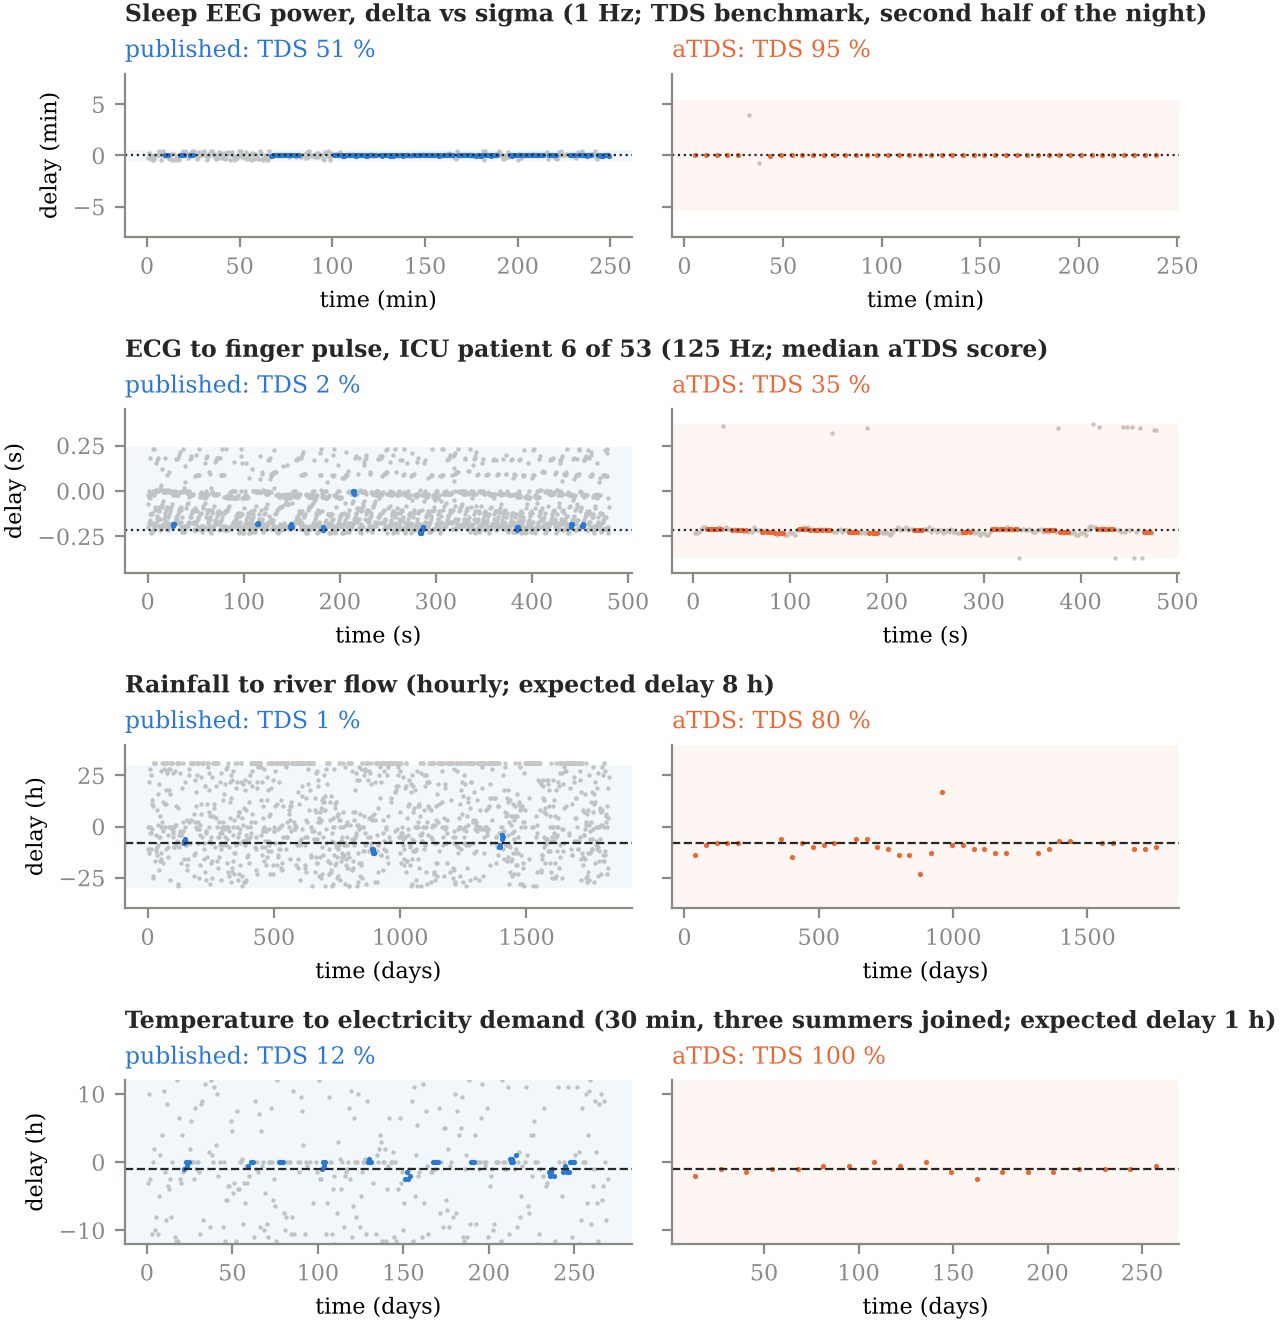
\includegraphics[width=\textwidth]{figures/fig_real_traces.png}
\caption{Delay found in each window ($\tau_0$) for four real records, published setting (left) and aTDS (right). Coloured: stable windows; grey: unstable windows; shaded band: the lag range searched (y-axes are zoomed; the aTDS lag ranges for river and electricity are $\pm40$ and $\pm13.5$ days). Dashed line: the delay expected from the domain (8\,h for rainfall to river flow, 1\,h for temperature to demand); dotted line: delay 0 for the EEG pair, and the full-record waveform alignment for the ECG pair. Negative delay: the first signal leads. EEG: parameters set on the first half of the night, scored on the second. ECG: the patient with the median aTDS score of 53. On the EEG pair both settings find the coupling; on the other three aTDS shows a continuous line of stable windows at the expected delay, while the published setting has few stable windows and its delays spread over its lag range.}
\label{fig:realtraces}
\end{figure}
\subsection{Physiological data}
\label{sec:res-physio}
\paragraph{Benchmark reproduction and a single sleep-EEG pair.}
\label{sec:res-benchmark}
The original MATLAB implementation of TDS gives 43.61\,\% for the benchmark pair of $\delta$- and $\sigma$-band EEG power (29\,941\,s at 1\,Hz) distributed with it. With the published setting and the causal stability anchor, pyTDS gives 43.53\,\%; with the default, non-causal anchor used everywhere else in this paper it gives 58.1\,\%. With parameters set on the first half of the night and scored on the second half, both settings detect the known strong coupling of this pair at delay 0: the published setting scores 50.8\,\% against a chance level of 1.2\,\% (95th percentile 2.6\,\%), and aTDS (window 652\,s, lag $\pm325$\,s, tolerance $\pm22$\,s) 95.5\,\% against 2.1\,\% (95th percentile 11.4\,\%); capped at 300\,s, aTDS scores 82.7\,\% against 2.3\,\%. Both are significant at the smallest $p$ possible with 100 rotations ($p \le 0.01$). With no ground truth beyond detection, this pair cannot rank the two settings; the cohort below can.

\paragraph{A new physiological test: heartbeat to finger pulse at 125\,Hz.}
\label{sec:res-bidmc}
Physiological TDS studies have mostly used signals resampled to 1\,Hz, the regime the published parameters were chosen for. To test aTDS on physiological data that TDS has not been applied to, we used the BIDMC PPG and Respiration data set on PhysioNet~\cite{Pimentel2017BIDMC,Goldberger2000PhysioNet}: 53 adult intensive-care recordings of 8 minutes at 125\,Hz with the ECG (lead II) and the finger photoplethysmogram (pulse). The two signals are coupled by physiology: each heartbeat produces a pulse wave that reaches the finger after the pulse arrival time, here a median of 0.53\,s (from the R peak to the steepest upstroke of the pulse, measured beat by beat; median heartbeat interval 0.64\,s). Both signals were band-pass filtered (ECG 0.5--30\,Hz, pulse 0.5--8\,Hz). True pairs are the ECG and pulse of the same patient (53); as uncoupled controls, the ECG of each patient was paired with the pulse of another patient (53 pairs, each pulse used once). aTDS was set on each pair on its own.

At 125\,Hz the published window of 60 samples is 0.48\,s, shorter than one heartbeat, and its lag range of $\pm0.24$\,s covers less than half a beat. It found the coupling in few patients: median score 1.6\,\% (control mean 1.2\,\%), 14 of 53 patients above the 95th percentile of the controls, AUC 0.69 (95\,\% interval 0.58--0.79). aTDS chose windows of 2.9--5.9\,s (median 4.3\,s, six to seven heartbeats) and a lag range of about half a heartbeat (median $\pm0.34$\,s, from the rhythm cap), without being told the sampling rate or the heart rate. It detected the coupling in 49 of 53 patients (median score 35\,\%; AUC 0.95, 0.90--0.99) and scored higher than the published setting in 47 of 53 (\cref{fig:bidmc}, \cref{tab:bidmc}). The controls also show that false stability stayed low: their mean aTDS score was 3.3\,\% (95th percentile 7.5\,\%). In 12 of the 53 true pairs the tolerance calibration could not reach the 5\,\% budget even at zero tolerance, because rotated copies of a heartbeat signal still line up with the ECG by chance; these pairs were scored with tolerance 0. Because the heartbeat repeats, a delay between these waveforms is only defined up to one beat, and TDS, which uses the absolute correlation, can also lock half a beat away. The aTDS delay agreed with the full-record alignment of the two waveforms within 0.04\,s in 40 of 53 patients and with the beat-by-beat pulse arrival time (modulo one beat) within 0.1\,s in 24 of 53 (median difference 0.07\,s); the published setting, where it found a delay, matched the pulse arrival time more closely (within 0.1\,s in 32 of the 41 patients with a delay), because its short window aligns the sharp ECG spike with the pulse upstroke rather than the whole waveforms. This test therefore shows detection on new physiological data at a new sampling rate; it is not a test of delay accuracy.

\begin{figure}[t]
\centering
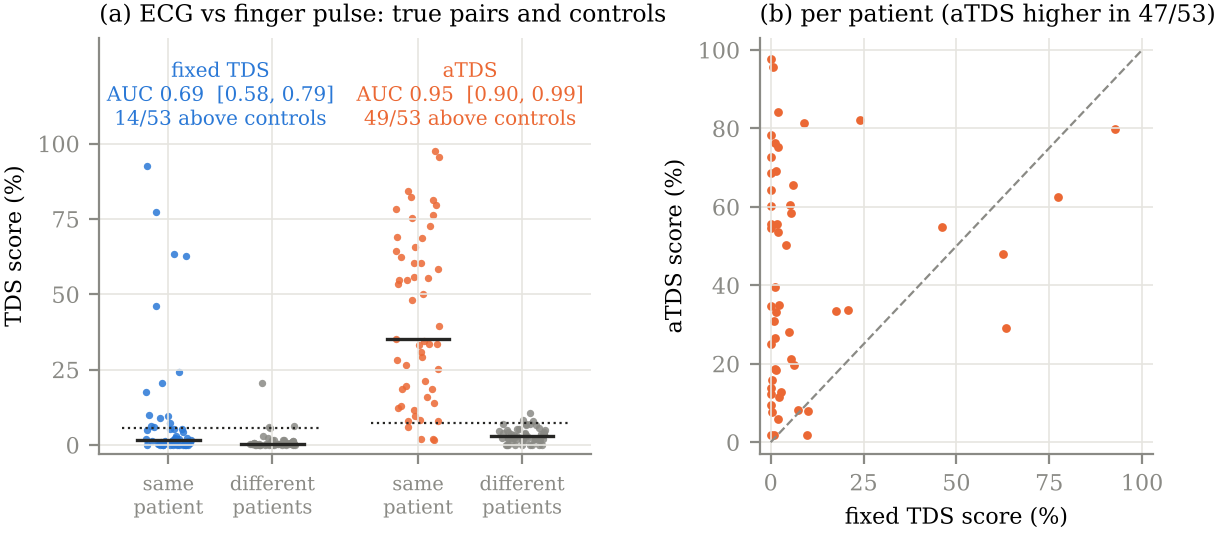
\includegraphics[width=\textwidth]{figures/fig_bidmc.png}
\caption{ECG and finger pulse in 53 intensive-care patients at 125\,Hz (BIDMC, PhysioNet). (a) TDS scores of true pairs (same patient) and controls (ECG and pulse of different patients); bars: medians; dotted: 95th percentile of the controls; AUC with bootstrap 95\,\% interval. (b) Score per patient, published vs aTDS; dashed: equal scores.}
\label{fig:bidmc}
\end{figure}

\begin{table}[t]
\centering
\caption{ECG and finger pulse at 125\,Hz, 53 intensive-care patients (BIDMC). Controls: ECG and pulse of different patients. Delay agreement is modulo one heartbeat.}
\label{tab:bidmc}
\footnotesize
\begin{tabular}{lcc}
\toprule
 & Published & aTDS \\
\midrule
Window / lag range / tolerance & 0.48\,s / $\pm0.24$\,s / $\pm8$\,ms & 2.9--5.9\,s / $\approx\pm0.34$\,s / mostly 0 \\
Median score, true pairs & 1.6\,\% & \textbf{35\,\%} \\
Mean score, controls (95th percentile) & 1.2\,\% (5.7\,\%) & 3.3\,\% (7.5\,\%) \\
AUC, true pairs vs controls [95\,\% interval] & 0.69 [0.58, 0.79] & \textbf{0.95} [0.90, 0.99] \\
Patients above the controls' 95th percentile & 14 / 53 & \textbf{49 / 53} \\
Patients with the higher score & 6 / 53 & \textbf{47 / 53} \\
Patients with a delay (3+ stable windows) & 41 / 53 & 53 / 53 \\
Delay within 0.1\,s of pulse arrival time & \textbf{32 / 41} & 24 / 53 \\
Delay within 0.04\,s of full-record alignment & 22 / 41 & \textbf{40 / 53} \\
\bottomrule
\end{tabular}
\end{table}


\paragraph{Sleep networks in a 35-subject cohort.}
\label{sec:res-cohort}
\paragraph{Data and design.} We analysed 35 overnight polysomnographic recordings prepared in the author's MSc project to reproduce the network analysis of Bashan et al.~\cite{Bashan2012NetworkPhysiology}. Each recording has 10 channels at 1\,Hz: heart rate, respiratory rate, the standard deviation of chin EMG, leg EMG and EOG, and the $\delta$, $\theta$, $\alpha$, $\sigma$ and $\beta$ EEG band powers; recordings last 23\,150--31\,752\,s and are scored into wake (W), light sleep (LS), deep sleep (DS) and REM. The cohort analysis uses the default, non-causal stability anchor. We compared three settings, each a single parameter set for the whole cohort: the published setting; aTDS, with the window from the median over subjects of $\max_i B_i$ (228) and the tolerance calibrated on rotations pooled over 50 random subject--pair combinations, giving $L = 2\,868$\,s (the 10\,\% cap), $\tau_{\max} = \pm1\,433$\,s and $\mathrm{tol} = \pm136$\,s; and aTDS with the window capped at 300\,s ($\tau_{\max} = \pm149$\,s, $\mathrm{tol} = \pm14$\,s). For each subject, each of the 45 links and each setting, the delay series and stability labels were computed over the whole night; a window was assigned to a stage if at least 80\,\% of its seconds carried that stage, and the per-stage TDS is the percentage of stable windows among those assigned (at least 3 required). Significance used the cross-subject, stage-matched null of the original studies~\cite{Bashan2012NetworkPhysiology}: for each link, 100 surrogate pairs combined channel $i$ of one subject with channel $j$ of another, scored with the first subject's stages, and a link was significant in a subject and stage if its TDS exceeded the 95th percentile of this null.

\paragraph{The uncapped window is too long for sleep staging.} With a 48-minute window, no subject had three windows lying at least 80\,\% inside wake, REM or deep sleep, and only 24 subjects had three in light sleep, so the uncapped setting cannot resolve sleep stages. This is the time-resolution limit noted in \cref{sec:conclusion} on real data: slow physiological signals ask for long windows, and stage-resolved analyses must cap them.

\paragraph{Stage contrasts.} \Cref{fig:cohort} and \cref{tab:cohort} compare the published setting with aTDS capped at 300\,s. Raw scores are higher under aTDS in every stage because its tolerance is wider, so they are not comparable across settings; the number of links significant against the stage-matched null is the fair comparison. Both settings show the strong light- versus deep-sleep contrast: mean link TDS, $d_z = 1.37$ (published) and 1.65 (aTDS), with light sleep higher in 91\,\% and 94\,\% of subjects; the gain, $+0.31$ (95\,\% interval $-0.06$ to $+0.75$), is not significant, and for significant links the gain is not significant either ($-0.14$, $-0.74$ to $0.47$). Under the published setting REM had lower mean link TDS than deep sleep ($d_z = -0.50$, interval $-0.88$ to $-0.17$), although it had more significant links ($d_z = 0.75$); under aTDS the mean-TDS inversion disappeared ($d_z = 0.11$, $-0.25$ to $0.42$; gain $+0.67$, $0.40$ to $0.98$), and the significant-link contrast was unchanged (gain $+0.15$, $-0.20$ to $0.50$). The wake contrast was weaker under aTDS ($d_z = 0.29$ vs 0.57 for mean TDS; for significant links, gain $-1.17$, $-1.65$ to $-0.77$), and it rests on 26 subjects only: 8 subjects lack three pure 300-s wake windows and one lacks deep-sleep windows. There is no ground truth for the REM ordering: the mean-TDS change may reflect the wider tolerance rather than physiology, and the significant-link contrast, which is calibrated against each setting's own null, did not change. We therefore do not count it as an improvement. On real staged data, aTDS does not sharpen sleep-stage contrasts: it reproduces the main contrast, leaves the significant-link contrasts unchanged or weaker, and loses power where stage episodes are short.

\begin{figure}[t]
\centering
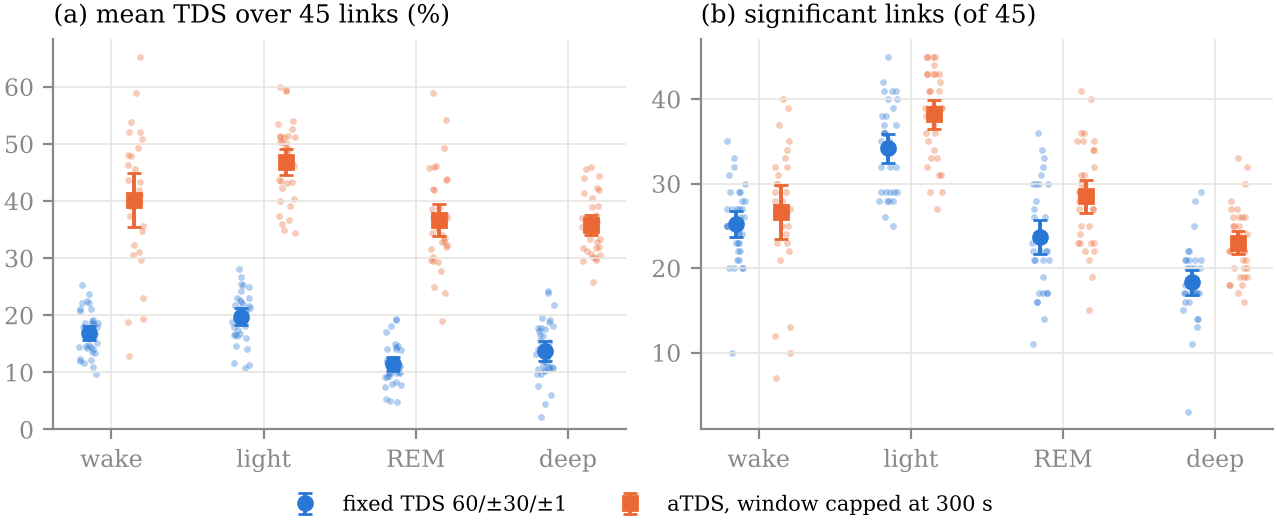
\includegraphics[width=\textwidth]{figures/fig_cohort_stages.png}
\caption{35 overnight recordings, 10 physiological signals, 45 links. (a) Mean TDS over the 45 links per subject and sleep stage; (b) number of links whose TDS exceeds the 95th percentile of the cross-subject, stage-matched null. Small dots: subjects; large markers: mean with 95\,\% interval. Scores of the two settings are not comparable in (a) because aTDS uses a wider tolerance; (b) is calibrated against each setting's own null.}
\label{fig:cohort}
\end{figure}

\begin{table}[t]
\centering
\caption{Sleep-stage contrasts in 35 subjects: paired effect size $d_z$ [95\,\% bootstrap interval] and share of subjects with a positive difference. Gain: aTDS (300\,s cap) minus published, paired. $n$ = subjects with enough stage windows (published: 35).}
\label{tab:cohort}
\footnotesize
\resizebox{\textwidth}{!}{%
\begin{tabular}{llccc}
\toprule
Measure & Contrast & Published & aTDS, 300\,s cap ($n$) & Gain \\
\midrule
Mean link TDS & LS $-$ DS & 1.37 [1.02, 1.91] (91\,\%) & 1.65 [1.27, 2.25] (94\,\%) (34) & $+0.31$ [$-0.06$, 0.75] \\
 & W $-$ DS & 0.57 [0.25, 0.97] (69\,\%) & 0.29 [$-0.09$, 0.76] (65\,\%) (26) & $-0.28$ [$-0.70$, 0.13] \\
 & REM $-$ DS & $-0.50$ [$-0.88$, $-0.17$] (40\,\%) & 0.11 [$-0.25$, 0.42] (47\,\%) (34) & $+0.67$ [0.40, 0.98] \\
 & LS $-$ REM & 1.90 [1.53, 2.53] (100\,\%) & 1.37 [0.97, 1.97] (91\,\%) (35) & $-0.53$ [$-1.18$, 0.05] \\
\midrule
Significant links & LS $-$ DS & 2.58 [2.11, 3.41] (100\,\%) & 2.47 [1.95, 3.34] (100\,\%) (34) & $-0.14$ [$-0.74$, 0.47] \\
 & W $-$ DS & 1.16 [0.69, 1.88] (89\,\%) & 0.34 [$-0.04$, 0.95] (69\,\%) (26) & $-1.17$ [$-1.65$, $-0.77$] \\
 & REM $-$ DS & 0.75 [0.45, 1.13] (74\,\%) & 0.88 [0.58, 1.25] (74\,\%) (34) & $+0.15$ [$-0.20$, 0.50] \\
 & LS $-$ REM & 1.67 [1.26, 2.40] (94\,\%) & 1.75 [1.35, 2.39] (94\,\%) (35) & $+0.08$ [$-0.48$, 0.54] \\
\bottomrule
\end{tabular}}
\end{table}


\paragraph{Stage-aware aTDS.}
\label{sec:res-stage}
The 300-s cap above was a choice, and the tolerance was calibrated on rotations that ignore stage structure. We therefore also derived both from the stages. Stage episodes had a median length of 300\,s over all stages (wake 90\,s, light sleep 420\,s, deep sleep 480\,s, REM 480\,s; 1\,573 episodes). The stage-aware setting used half the median episode length as window, $L = 150$\,s ($\tau_{\max} = \pm74$\,s), and calibrated a tolerance \emph{per stage} on 50 cross-subject, stage-matched surrogates with the same rule (mean + 2 SE $\le 5$\,\%), giving $\pm6$\,s for wake, light and deep sleep and $\pm4$\,s for REM. With this setting 33 subjects contributed to the wake contrast (26 with the 300-s cap). All contrasts kept the signs of the published setting: mean link TDS $d_z = 1.62$ (light vs deep), 0.53 (wake vs deep), $-0.70$ (REM vs deep) and 2.16 (light vs REM). None of the gains over the published setting was significant (mean link TDS: $+0.28$, interval $-0.01$ to $0.57$, for light vs deep; $+0.26$, $-0.21$ to $0.88$, for light vs REM), and in significant links the wake contrast was again weaker ($-1.02$, $-1.48$ to $-0.68$). Stage-aware calibration thus removes the arbitrary cap and the rotation null from the sleep analysis without changing its conclusion: on 1-Hz sleep networks, the regime for which the published parameters were chosen, aTDS does not improve on them.


\subsection{Data from other fields: rivers, electricity and fuel prices}
\label{sec:res-fields}
To test whether the rules transfer beyond physiology, we applied both settings to public records from three fields, including three river catchments of the same hydrological data set (airGR catchments L0123001--L0123003), whose delays are known from the domain (a catchment's response time, the thermal response of demand) and, more precisely, from the peak of the full-record cross-correlation---a partly circular reference, since the cross-correlation is itself a delay estimator: hourly catchment rainfall and river flow (43\,848\,h, airGR catchment L0123003), half-hourly Melbourne temperature and Victoria electricity demand in summer after removing the mean daily profile (13\,008 half-hours), and weekly changes of the WTI crude-oil price and US retail gasoline price (1\,746 weeks). aTDS was calibrated on rotations of each record itself; significance used 200 rotations (\cref{tab:fields}, \cref{fig:fields}).

\begin{table}[t]
\centering
\caption{Records from other fields (hydrology: three airGR catchments; energy; fuel prices). Score vs the 95th percentile of 200 rotated copies (null95); delay = most frequent $\tau_0$ among stable windows, signed so that the driver (rain, temperature, crude oil) leads.}
\label{tab:fields}
\footnotesize
\resizebox{\textwidth}{!}{%
\begin{tabular}{lllcccc}
\toprule
Record & Known delay & Setting & Parameters ($L$ / $\tau_{\max}$ / tol) & Score (null95) & $p$ & Delay found \\
\midrule
Rainfall $\to$ river flow, hourly & about 8\,h & published & 60\,h / 30\,h / 1\,h & 1.2\,\% (1.1) & 0.02 & 13\,h (wrong) \\
 & & aTDS & 79.8\,d / 39.8\,d / 1.8\,d & 79.5\,\% (9.1) & 0.005 & \textbf{8\,h} \\
Rainfall $\to$ river flow, daily (L0123001) & 0--3 days & published & 60 / 30 / 1 days & 59.1\,\% (2.6) & 0.005 & 1 day \\
 & & aTDS & 501 / 250 / 20 days & 97.6\,\% (12.3) & 0.005 & 2 days \\
Rainfall $\to$ river flow, daily (L0123002) & 1 day (weak xcorr peak) & published & 60 / 30 / 1 days & 32.4\,\% (2.3) & 0.005 & 1 day \\
 & & aTDS & 1\,059 / 367 / 9 days & 21.1\,\% (21.1) & 0.10 & 162 days (wrong) \\
Temperature $\to$ electricity demand & about 1\,h & published & 30\,h / 15\,h / 30\,min & 11.8\,\% (3.0) & 0.005 & 0 (wrong) \\
 & & aTDS & 27.1\,d / 13.5\,d / 1.0\,d & 100\,\% (21.1) & 0.005 & \textbf{1\,h} \\
Crude oil $\to$ gasoline, weekly changes & 1--2 weeks & published & 60 / 30 / 1 weeks & 86.0\,\% (7.0) & 0.005 & 0 weeks \\
 & & aTDS & 64 / 31 / 3 weeks & 92.5\,\% (15.1) & 0.005 & 0 weeks \\
\bottomrule
\end{tabular}}
\end{table}

On the two daily catchments the published 60-day window already fits the time scale: on L0123001 both settings find the expected 0--3-day delay (1 and 2 days), and on L0123002 aTDS fails (not significant, $p = 0.10$; delay 162 days), whereas the published setting reports 1 day, consistent with the weak positive cross-correlation peak ($r = 0.054$ at +1 day). On the hourly, energy and fuel records both settings detect coupling, the published setting only marginally for rainfall--runoff (1.2\,\% vs a null95 of 1.1\,\%, $p = 0.02$). aTDS reports the known delay for rainfall--runoff (8\,h) and temperature--demand (1\,h), where the published setting, whose 60-sample window is short against these slow signals, reports 13\,h and 0. For the oil--gasoline record both settings report no delay: in weekly changes the cross-correlation already peaks at lag 0 ($r = 0.55$, partly because WTI and retail prices are recorded on different weekdays; lag 1: $r = 0.39$), so a 1--2-week delay is not resolved at this sampling, and the record does not discriminate between the settings. The aTDS windows (80 and 27 days) are long, which is acceptable here because the delays are constant over the records.

\begin{figure}[t]
\centering
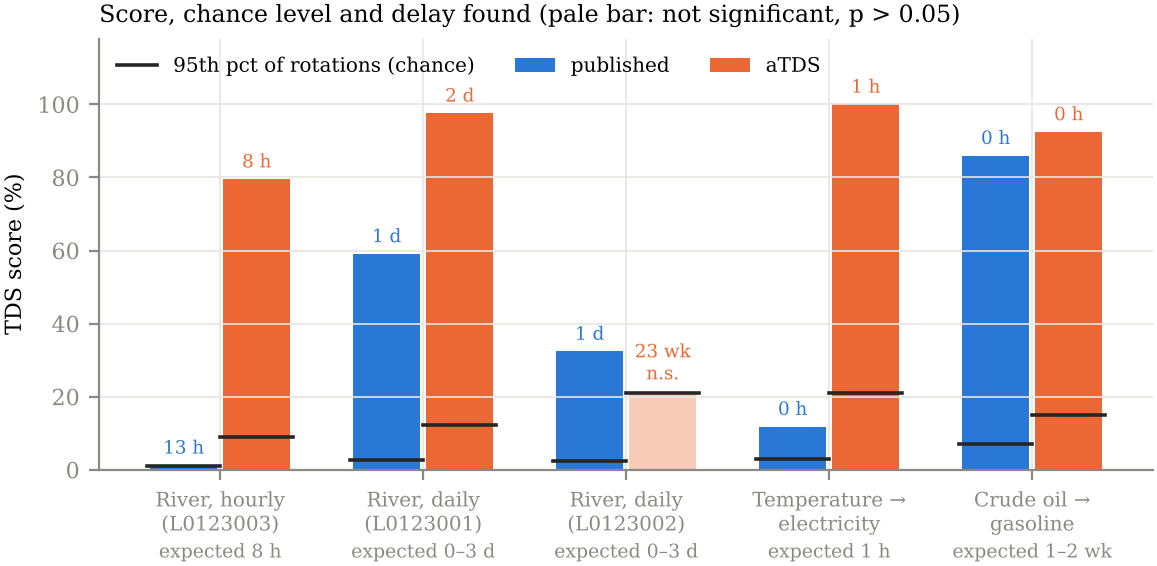
\includegraphics[width=\textwidth]{figures/fig_fields_significance.png}
\caption{Records from other fields: TDS score per setting (bars), the 95th percentile of 200 rotated copies (black lines, the chance level) and the delay found (above the bars). Pale bar: not significant ($p > 0.05$). Expected delays below each record.}
\label{fig:fields}
\end{figure}

\paragraph{The failing catchment.} The failing catchment L0123002 has a strongly seasonal river flow (autocorrelation 0.62 at a lag of one year); the first-zero Bartlett factor of the flow (38.8) ignores the seasonal lobe and gives a window of about three years with only 19 windows, of which 4 were stable, so the score (21.1\,\%) equalled the 95th percentile of the rotation null. Capping the window at 120 days recovered the 1-day delay (score 10.3\,\% vs null95 7.4\,\%, $p = 0.015$); capping it at 365 days did not (no stable window). Seasonal signals, like rhythmic ones, need a cap below the seasonal period.



\section{Part 4: conclusion}
\label{sec:conclusion}
\Cref{tab:scoreboard} collects every comparison of the paper between aTDS and the published setting.

\begin{table}[t]
\centering
\caption{Scoreboard: every comparison in this paper between the published setting (60 / $\pm30$ / $\pm1$ samples) and aTDS. ``Better'' and ``worse'' require non-overlapping 95\,\% intervals or a clear difference in counts; otherwise ``equal''.}
\label{tab:scoreboard}
\footnotesize
\begin{tabularx}{\textwidth}{>{\raggedright\arraybackslash}p{4.3cm}>{\raggedright\arraybackslash}X>{\raggedright\arraybackslash}X>{\raggedright\arraybackslash}p{1.25cm}}
\toprule
Test & Published & aTDS & aTDS is \\
\midrule
\multicolumn{4}{l}{\emph{Part 1: each rule on its own}} \\
Window, 4$\times$ slower system & AUC 0.51 & 0.79 & better \\
Lag range, delays beyond 30 samples & wrong delay in 50 / 50 (16 wrong sign) & right in 50 / 50 & better \\
Tolerance, $r = 8$ (delay found) & 66\,\% & 85\,\% & better \\
Tolerance, chance score on new data & -- & 3.3--4.4\,\% (budget 5\,\%) & as designed \\
\midrule
\multicolumn{4}{l}{\emph{Part 2: simulated data}} \\
Slow-down, $r = 1$ (published scale) & AUC 0.997 & 0.995 & equal \\
Slow-down, $r = 2$ / 4 / 8 & 0.89 / 0.59 / 0.54 & 0.98 / 0.92 / 0.88 & better \\
Slow-down, $r = 16$ & 0.51 & 0.65 & better \\
Long memory, $H = 0.6$ / 0.75 & 0.60 / 0.70 & 0.59 / 0.65 & equal \\
Long memory, $H = 0.9$ & 0.46 & 0.82 & better \\
Rhythm, $d = 8$ & 0.97, delay 43\,\% & 1.00, 100\,\% & better \\
Rulkov neurons, $d = 16$ / 32 & 0.73 / 0.79 & 1.00 / 1.00 & better \\
Changing dynamics, 2nd half & 0.71, delay 45\,\% & 0.96, 90\,\% & better \\
Coupling that switches (regime A stable) & 5.6\,\% & 98.9\,\% & better \\
\quad false stability in uncoupled regime & 0.9\,\% & 8.1\,\% (3.8\,\% with margin) & worse \\
Drifting delay (stable windows) & 8.5\,\% & 86.5\,\% & better \\
Monotone nonlinear coupling & AUC 0.997 & 1.0 & equal \\
Non-monotone coupling & 0.80 & 0.75 & equal \\
\midrule
\multicolumn{4}{l}{\emph{Part 3: real data}} \\
EEG benchmark pair & detected (50.8\,\%) & detected (95.5\,\%) & equal \\
35-subject sleep cohort, stage contrasts & reproduced & reproduced, no gain & equal \\
ECG $\to$ finger pulse, 125\,Hz, 53 patients & AUC 0.69, 14 / 53 & 0.95, 49 / 53 & better \\
\quad delay vs pulse arrival time & 32 / 41 & 24 / 53 & worse \\
Rainfall $\to$ river, hourly & 13\,h (wrong) & 8\,h (right) & better \\
Rainfall $\to$ river, daily L0123001 & 1 day & 2 days & equal \\
Rainfall $\to$ river, daily L0123002 & 1 day & not significant & worse \\
Temperature $\to$ electricity & 0 (wrong) & 1\,h (right) & better \\
Crude oil $\to$ gasoline & 0 weeks & 0 weeks & equal \\
\bottomrule
\end{tabularx}
\end{table}

\paragraph{What aTDS is.} aTDS is Time Delay Stability with its three parameters set by the signals instead of by hand: a window that holds 30 independent samples of the slowest signal, a lag range of half the window (capped at half a rhythm period), and the widest tolerance whose chance score on coupling-free, rotated copies of the same signals stays within a 5\,\% false-stability budget. The 4-of-5 stability rule of the original method is unchanged, and no rule uses which pairs are coupled or what the delay is.

\paragraph{Why it is needed.} The published parameters are counted in samples and were chosen for 1-Hz sleep recordings. On any other time scale or sampling rate they hold too little information per window, search too narrow a lag range and accept too little wobble of the delay. The result is not only lower detection but silent errors: a fixed lag range returned high TDS scores (72--96\,\%) with wrong delays, some of them with the wrong sign, and the published setting lost almost all detection once the system was four times slower than it assumes.

\paragraph{Verdict.} aTDS does what it was designed to do. Each of its three rules was tested on its own and works: the window keeps the information per window constant, the lag range reports the true delay where a fixed range fails, and the tolerance keeps false stability within its budget on new data. On simulated signals aTDS restores detection and correct delays where the published setting fails, follows coupling that switches with the regime and delays that drift. On real data it reproduces the original TDS benchmark, detects the physiological network of 35 sleep recordings and reproduces the known sleep-stage pattern---agreeing with the published parameters exactly where they were designed to fit---on ECG and finger-pulse recordings at 125\,Hz, which, to our knowledge, TDS had not been applied to, it detects the heart-to-pulse coupling in 49 of 53 patients against 14 with the published setting; and it finds the known delays in river and electricity records where the published setting does not. aTDS makes TDS a reproducible tool for any system and sampling rate, with a stated false-alarm budget.

\paragraph{Limitations.} aTDS scales the parameters; it does not optimise them: with permanent coupling, longer windows detect better, and an oracle tuned on labelled data did better. Because matching the time scale is what matters, any rule that tracks it helps: in our simulations, multiplying the published parameters by a factor estimated from the correlation time performed similarly to aTDS on the slow-down test. This is expected and supports the premise of aTDS rather than weakening it; aTDS in addition sets the lag range and the tolerance from the data with a stated false-alarm budget instead of copying the published ratios. Full-record delay estimators are better when the delay is constant and the coupling always on. On 1-Hz sleep networks aTDS brought no gain over the published setting, which was designed for them, and the uncapped window was too long to resolve sleep stages, so stage-resolved analyses need a window cap. Near the boundaries of coupled regimes, long windows inherit stability (8--9\,\% false stability without a boundary margin). The calibrated tolerance grows with the time scale, so aTDS scores should be compared with the aTDS chance level of the same data, not with published TDS values. Seasonal and rhythmic signals need a window cap below their period, and correlation-based TDS does not capture non-monotone coupling.

\section*{Code and data availability}
pyTDS, the aTDS experiment scripts, their raw results (JSON) and the figure scripts are available at \url{https://github.com/Marku-a/pyTDS}. All random seeds are fixed. The 35 polysomnographic recordings are research data that are not redistributed; only derived results are published. The rainfall--runoff, electricity-demand and fuel-price records are public (sources in \texttt{experiments/atds\_real/data\_fields/MANIFEST.json}). The ECG and finger-pulse recordings are the public BIDMC data set on PhysioNet (\url{https://physionet.org/content/bidmc/1.0.0/}); the analysis is \texttt{experiments/atds\_real/bidmc.py}.


\section*{Use of AI tools}
This manuscript was drafted with AI assistance (Claude, using the PaperOrchestra writing pipeline) from the author's method description, experiment scripts and raw results; all numbers were checked against the raw results. All TDS computations use the author's pyTDS.

%%%%%%%%% REFERENCES %%%%%%%%%
\bibliographystyle{unsrtnat}
\bibliography{references}
%%%%%%%%% REFERENCES %%%%%%%%%

\end{document}
